\documentclass[../thesis]{subfiles}

\begin{document}
	\section{Further Optimizations}
	\label{sec:mic:further}

	One of the most problematic issues when using a \numa system lies in the fact that a process that starts in one processor may at some time be scheduled out and moved to another. The problem behind this lies in memory hierarchy. Since the process started in a specific processor, it populated the cache and filled the memory directly linked to that processor with the data it requires. When moved to another, its data is no longer available in cache, which leads to a memory access, but the data it requires no longer lies in the closest memory. This also happens at the core level, with threads being scheduled to different cores inside the same processor, losing the advantage of locality in the core's private cache. For the specific case of \intel\mic devices, it is important for threads working with consecutive elements or in the same block to be in the same core in order to maximize the efficiency of the cache.

	Although OpenMP (specification 3.1) does not include any way to control thread affinity, \intel's OpenMP library was later found to contain a mechanism for it through an environment variable (\texttt{KMP\_AFFINITY}) \cite{PRACE:MIC:BestPracticeGuide,CESGA:MIC:Evaluation}. It is expectable that a balanced affinity policy, where the threads are spread amongst the cores but grouped sequentially by ID when the number of demanded threads exceeds the number of cores, with any granularity would achieve higher efficiency due a better usage of the first levels of cache.

	\begin{figure}
		\begin{center}
			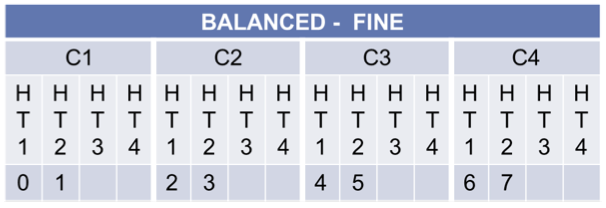
\includegraphics[width=\textwidth]{assets/images/kmp_affinity_balanced.png}
		\end{center}
		\caption{Example of balanced policy in a 4 core coprocessor for 8 threads with granularity fine (source: \cite{CESGA:MIC:Evaluation})}
		\label{fig:kmp_affinity:balanced}
	\end{figure}

	Rerunning the performance tests at this point with the correct affinity setup would hamper the development of a \cuda implementation (described in the next chapter). Consequently, it is left for future work.

\end{document}
